% !TEX root = master.tex
\chapter{Aufbau und Bedienbarkeit (Frontend)}
\label{ch:a-frontend}

Das Frontend von GuardX folgt durchg\"angig der klassischen Struktur aus Kopfbereich mit
Navigation, Inhaltsbereich und Footer. Gestalterisch kommt ein dunkles \enquote{Cyber-Theme}
mit gr\"unen Akzenten zum Einsatz, das auf allen Seiten \"uber eine gemeinsame Stylesheet-Basis
(\texttt{style/main.css}, \texttt{style/navbar.css}) erzeugt wird.

\section{Navigation}
Die Navigation ist sowohl \emph{dynamisch} als auch \emph{responsiv} umgesetzt. Serverseitig
wird in jedem Seitenaufruf \"uber die Funktion \texttt{is\_mobile()} anhand des User-Agents
entschieden, ob die Desktop-Navigation (\texttt{template/navbar.php}) oder die mobile Variante
mit Hamburger-Men\"u (\texttt{template/navbar\_mobile.php}) eingebunden wird. Die angezeigten
Men\"upunkte h\"angen zus\"atzlich vom Login-Status und der Rolle ab: Nicht angemeldete Nutzer
sehen einen \emph{Login}-Punkt, angemeldete Nutzer den Bereich \emph{Mein Bereich} und
Administratoren zus\"atzlich \emph{System Admin}. Die Links werden \"uber die Hilfsfunktion
\texttt{get\_url()} erzeugt, damit sie unabh\"angig vom Installationsverzeichnis korrekt
aufl\"osen.

\begin{figure}[htbp]
    \centering
    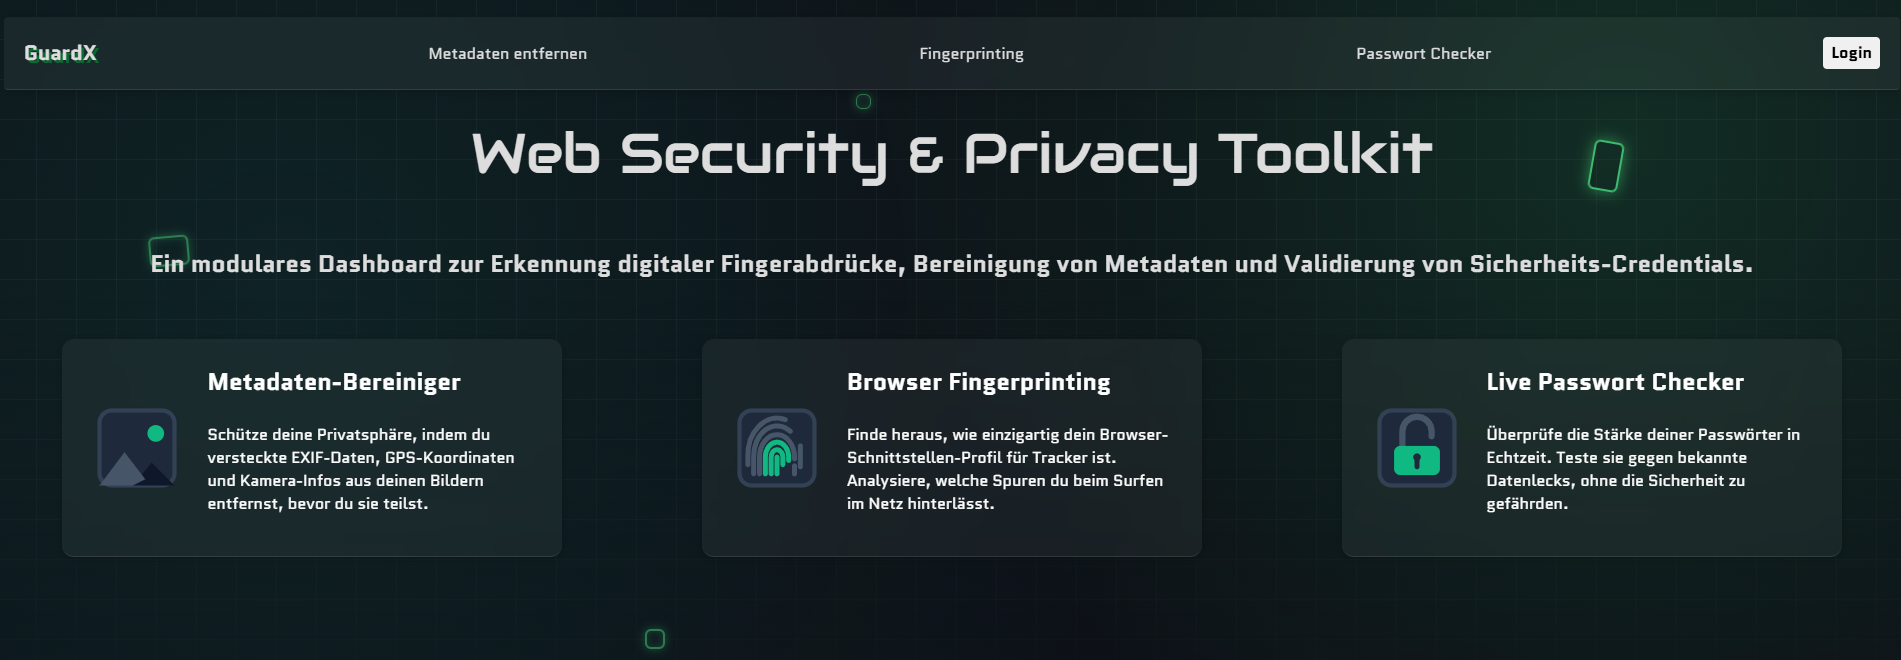
\includegraphics[width=0.8\textwidth]{img/navigation.png}
    \caption{Startseite (Dashboard) mit Desktop-Navigation und den drei Modulkacheln}
    \label{fig:a-start}
\end{figure}

\section{Startseite}
Die Startseite (\texttt{index.php}) dient als Dashboard und stellt die drei Fachmodule als
Kacheln mit kurzer Beschreibung vor: Metadaten-Bereiniger, Browser-Fingerprinting und
Live-Passwort-Checker. Von hier aus gelangt man per Klick direkt in das jeweilige Modul.

\section{Registrierung, Login und gesch\"utzte Bereiche}
\"Uber \texttt{auth.php} erfolgen Registrierung und Login in einem gemeinsamen, umschaltbaren
Formular. Nach erfolgreichem Login wird der Nutzer rollenabh\"angig weitergeleitet -- als Admin
in das Admin-Dashboard, sonst in den pers\"onlichen Bereich. R\"uckmeldungen (Erfolg, Fehler,
Sperrhinweise) werden direkt am Formular angezeigt.

Der \textbf{pers\"onliche Bereich} (\texttt{user.php}) erlaubt das \"Andern der E-Mail-Adresse
und des Passworts (mit Best\"atigung des aktuellen Passworts) sowie das L\"oschen des eigenen
Accounts. Sicherheitskritische Aktionen werden \"uber einen Best\"atigungsdialog abgesichert.

Der \textbf{Admin-Bereich} (\texttt{admin.php}) bietet eine tabellarische Benutzer\"ubersicht
mit Inline-Formularen, \"uber die Administratoren neue Benutzer anlegen, E-Mail-Adressen und
Passw\"orter setzen, die Rolle umschalten und Benutzer l\"oschen k\"onnen. Der eigene Account ist
gegen versehentliches L\"oschen gesch\"utzt.

\begin{figure}[htbp]
\centering
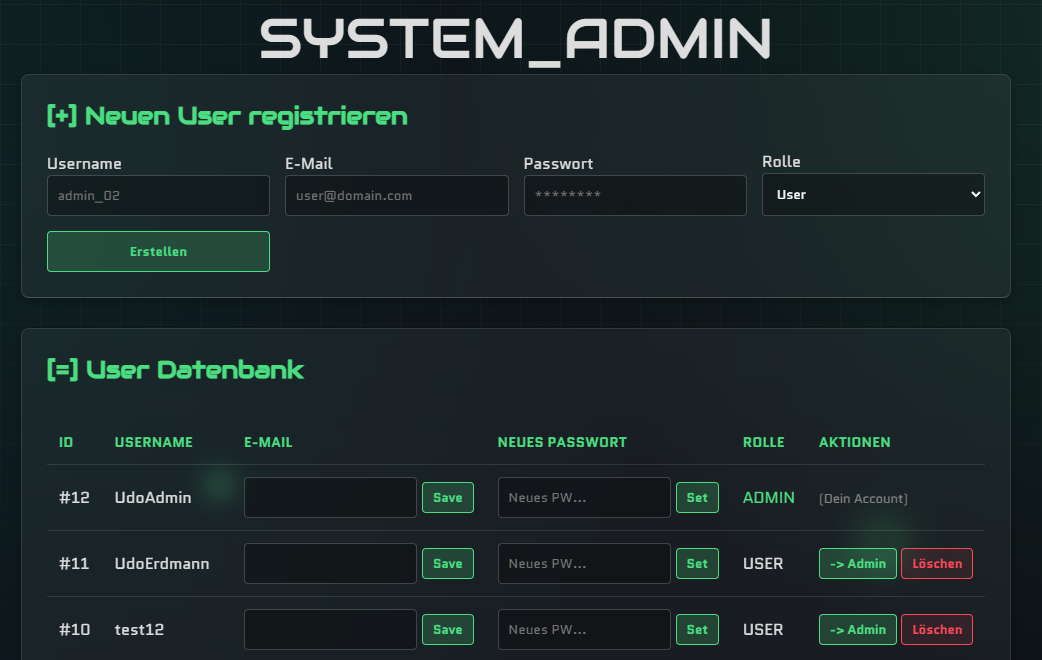
\includegraphics[width=0.8\textwidth]{img/admin-dashboard.png}
\caption{Admin-Bereich mit Benutzerverwaltung}
\label{fig:a-admin}
\end{figure}

\section{Fachmodule}
\textbf{Metadaten-Bereiniger.} \"Uber ein Upload-Formular wird ein Bild hochgeladen; die
Anwendung liest die \ac{exif}-Daten aus, bietet sie als \ac{json}-Datei zum Download an und
liefert eine von Metadaten bereinigte Kopie des Bildes zur\"uck. Das Original wird nach der
Verarbeitung serverseitig gel\"oscht.

\textbf{Browser-Fingerprinting.} Die Seite (\texttt{info.php}) stellt anschaulich dar, welche
Merkmale einen Browser identifizierbar machen (u.\,a. Canvas- und WebGL-Fingerprint, Zeitzone,
Sprache, Hardware). Die Werte werden clientseitig per JavaScript ermittelt und hervorgehoben.

\textbf{Live-Passwort-Checker.} Bei jeder Eingabe wird das Passwort per \ac{ajax} an den Server
geschickt und sofort bewertet: Die Anforderungen an die St\"arke (L\"ange, Gro\ss-/Kleinbuchstaben,
Ziffern, Sonderzeichen) werden mit regul\"aren Ausdr\"ucken gepr\"uft, zus\"atzlich erfolgt ein
datenschutzfreundlicher Abgleich gegen bekannte Datenlecks. Ein Auge-Symbol blendet das Passwort
bei Bedarf ein.

\section{Meldungen und Dialoge}
F\"ur Hinweise und Best\"atigungen werden zwei Mechanismen verwendet: einfache
\texttt{confirm()}-Dialoge f\"ur destruktive Aktionen (z.\,B. Benutzer l\"oschen) sowie ein
modaler jQuery-UI-Dialog, der vor Ablauf der Session erscheint und die Wahl zwischen
\emph{Bleiben} und \emph{Ausloggen} bietet.
